\section{Implementarea}

Implementarea \gls{wte} se bazează pe cod scris în limbajele Python, pentru nucleul simulatorului, ce implementează infrastructura și pe cod scris în limbajul C, pentru serverul \gls{netconf}, soluţia \gls{dvm} ce a fost dezvoltată anterior fiind adaptată pentru noua abordare. Codul este oferit cu sursă deschisă și poate fi găsit pe platforma GitHub~\cite{wte2017}. Paragrafele următoare vor prezenta detalii despre implementare, evidenţiind avantajele acestei abordări și motivele pentru care soluţia poate fi considerată un adevărat simulator de rețele de transport de date fără fir. 

\subsection{Fişierele de configurare}

\gls{wte} folosește fişiere de configurare, pentru a oferi o interfață simplă de configurare utilizatorilor. Există două fişiere scrise în limbajul \gls{json}, \textit{topology.json} și \textit{config.json}, primul pentru descrierea topologiei care va fi simulată și celălalt pentru a descrie caracteristicile configurabile ale simulatorului. Din aceeaşi categorie fac parte și modelele informaționale. Fişierele \gls{yang} asociate acestora sunt folosite de către simulator pentru a fi expuse de serverul \gls{netconf}.

Fişierul \gls{json} care descrie topologia are un format static, ce va fi prezentat în continuare. Acesta este ilustrat și în Figura~\ref{fig:wte_topology_json}.

\begin{figure}[h]
	\centering
	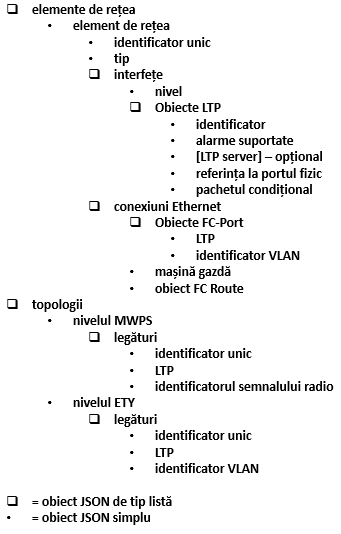
\includegraphics{wte_topology_json}
	\caption{Formatul fișierului JSON care descrie topologia rețelei simulată cu WTE.}
	\label{fig:wte_topology_json}
\end{figure}

Pentru descrierea topologiei unei rețele este suficient să cunoaştem dispozitivele și legăturile dintre acestea. Fiind rețele de transport de date fără fir, în cele mai simple cazuri, putem avea două tipuri de legături între echipamente: fără fir, sau legături Ethernet. Astfel, fişierul de topologie conţine două obiecte \gls{json} de tip listă: (i) \textbf{elemente de rețea} (\textit{network-elements}), ce descrie dispozitivele de rețea și (ii) \textbf{topologii} (\textit{topologies}), reprezentând legăturile dintre echipamente.

Fiecare element de rețea va avea mai multe detalii prezente în fişierul de topologie. Identificatorul unic reprezintă un nume unic ce va fi dat fiecărui dispozitiv de rețea, pentru a-l putea recunoaşte în topologia simulată. Tipul elementului se referă la soluţia ce va fi folosită pentru implementarea serverului \gls{netconf} ce va expune modelele informaționale dorite. În cazul alegerii \gls{dvm}, valoarea acestui element este \textit{OpenYuma}. Pentru cea de-a patra demonstraţie de concept \gls{onf}, o companie a folosit simulatorul \gls{wte} pentru dezvoltarea de aplicații \gls{sdn}, dar a preferat o soluție mai simplă, dar cu mai puţine capabilităţi pentru implementarea serverului \gls{netconf}, astfel că a folosit acest parametru pentru a informa nucleul simulatorului să folosească celălalt server. 

Elementul cel mai important al unui dispozitiv de rețea este reprezentat de obiectul \gls{json} de tip listă \textit{interfețe}, fiind responsabil pentru descrierea interfeţelor acelui dispozitiv. O interfață a unui echipament are ca echivalent un obiect \gls{ltp} din modelul informațional de bază. Obiectul \textit{nivel} din lista de interfețe reprezintă nivelul de transport asociat obiectului \gls{ltp}. Valorile pe care acesta le poate lua sunt descrise în modelul informațional de bază, în Capitolul~\ref{ch:sdn_in_contextul_wt}: \gls{mwps}, \gls{mws}, \gls{etc}, \gls{ety} și \gls{eth}. Fiecare interfață prezintă câteva detalii de care simulatorul are nevoie: identificatorul obiectului \gls{ltp}, alarmele suportate (simulatorul are nevoie de această valoare, deoarece în modelul informațional pentru microunde, pe baza acestui atribut este definită lista alarmelor suportate și aceasta are un număr minim elemente; dacă nu este implementat acest număr minim, modelul \gls{yang} prezentat de serverul \gls{netconf} nu va fi valid), obiectul \gls{ltp} care reprezintă serverul pentru obiectul \gls{ltp} curent, dacă există (pentru reprezentarea relaţiilor de tip client-server dintre interfețe), referinţa la portul fizic și pachetul condiţional folosit de acest obiect \gls{ltp}.

Următorul obiect \gls{json} care face parte din fişierul de descriere a topologiei este tot un obiect de tip listă, \textit{conexiuni Ethernet}. Acestea reprezintă obiectele \gls{fc} definite în modelul informațional de bază. Practic, acestea exprimă conexiunile interne între interfeţele dispozitivului (de exemplu, traficul de pe o interfaţă radio R1 va fi dirijat către o interfață Ethernet E2). De aceea, obiectul \textit{conexiuni Ethernet} conţine două obiecte de tipul porturi \gls{fc}, care descriu exact această legătură internă. Obiectul \gls{json} \textit{mașină gazdă} care este prezent aici este folosit pentru simularea unei gazde care folosește această conexiune internă și este utilizat pentru generarea sau recepţionarea de trafic în cadrul simulatorului.

Obiectul \gls{json} \textit{topologii} descrie legăturile dintre dispozitivele de rețea. Există două niveluri de transport la care pot exista aceste conexiuni: \gls{mwps}, adică legăturile fără fir și \gls{ety}, reprezentând conexiunile Ethernet dintre echipamente. Fiecare legătură este reprezentată ca un obiect \gls{json} de tip listă, având doar două elemente, ce descriu cele două capete ale conexiunii, prin identificatorul unic al dispozitivului și identificatorul unic al interfeţei.

Cel de-al doilea fişier \gls{json} folosit de \gls{wte} este \textit{config.json}. Formatul acestuia poate fi observat în Figura~\ref{fig:wte_config_json}.

\begin{figure}[h]
	\centering
	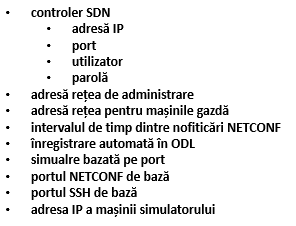
\includegraphics{wte_config_json}
	\caption{Formatul fişierului JSON de configurare a simulatorului WTE.}
	\label{fig:wte_config_json}
\end{figure}

Acesta conţine detaliile de conectare la echipamentul de control \gls{sdn}, în cazul în care se doreşte înregistrarea automată a dispozitivelor simulate la controler, constând în adresa \gls{ip}, portul, numele de utilizator și parola folosite pentru autentificare. Următorul parametru descrie adresa rețelei de administrare care să fie folosită pentru alocarea adreselor \gls{ip} pentru interfeţele de administrare ale echipamentelor simulate. În același mod se poate configura și plaja de adrese \gls{ip} care să fie alocată maşinilor gazdă, folosite pentru generarea și recepţionarea traficului de date prin rețeaua simulată. 

Echipamentele simulate pot genera, la fel ca \gls{dvm}, notificări \gls{netconf} fictive. Intervalul de timp dintre două astfel de notificări este prezent în fişierul \gls{json} de configurare. Parametrul \textit{înregistrare automată în \gls{odl}} este folosit de către utilizator pentru a configura simulatorul să facă sau nu înregistrarea automată a dispozitivelor în echipamentul de control specificat prin detaliile de conectare anterioare. Metoda de înregistrare folosită este specifică echipamentului de control \gls{odl}, dar poate fi extinsă și pentru altele.

Următorii parametri sunt folosiţi în cazul în care utilizatorul nu doreşte adrese \gls{ip} diferite pentru administrarea dispozitivelor simulate. Astfel, echipamentele vor putea fi accesate prin adresa \gls{ip} a maşinii pe care rulează simulatorul, dar prin porturi diferite. De aceea, este nevoie ca utilizatorul să configureze portul de bază (portul de la care începe numărătoarea în momentul asignării porturilor pentru fiecare element de rețea simulat), pentru protocoalele \gls{netconf} și \gls{ssh}.

\subsection{Adaptarea DVM pentru WTE}

Folosirea \gls{dvm} fără o adaptare prealabilă la cerințele \gls{wte} nu ar fi fost posibilă. În primul rând, \gls{dvm} a fost transformat astfel încât să poată fi folosit într-un container \textit{docker}. Cerinţa pentru \gls{dvm} a fost să permită rularea mai multor instanţe, fiecare în containerul \textit{docker} asociat, însă având o configuraţie proprie la dispoziţie, în funcție de detaliile cuprinse în fişierul de descriere a topologiei.

Am decis astfel împărțirea atributelor prezente în modelele informaționale de bază și pentru microunde în două tipuri: de configurare și de stare. Dacă în versiunile anterioare, baza de stocare de date de execuţie se construia manual, pentru toate atributele, în codul C al serverului \gls{netconf}, această abordare nu ar mai fi fost posibilă, deoarece configurația era variată pentru diferitele dispozitive de rețea ce trebuie simulate. Am dezvoltat astfel o soluție automată care să construiască această bază de stocare de date de execuţie \gls{netconf}. În cazul atributelor de configurare, soluţia a fost folosirea unui fişier \gls{xml} care să le conţină, împreună cu conceptul bazei de stocare de date de iniţializare. Astfel, în momentul în care serverul \gls{netconf} porneşte, va încărca în baza de stocare de date de execuţie conţinutul acelui fişier de iniţializare. Dacă structura fişierului \gls{xml} este corectă, serverul \gls{netconf} va expune interfeţele și celelalte detalii oferite de atributele de configurare către echipamentul de control \gls{sdn}. Această soluție înseamnă, din punctul de vedere al nucleului \gls{wte}, construirea acelui fişier \gls{xml} astfel încât să aibă o structură corectă și să reflecte informaţiile din fişierul care descrie topologia ce trebuie simulată.

În cazul atributelor de stare, am renunţat la abordarea folosită anterior pentru \gls{dvm}, și anume împărțirea acestora în atribute de execuţie și de iniţializare, deoarece nu s-ar fi putut aplica într-o manieră automată. Soluția în acest caz a fost modificarea uneltei oferite de cadrul software \textit{OpenYuma}, care generează scheletul codului C din fişierul *.yang asociat modelului informațional. Acesta a fost alterat astfel încât să preia valoarea oricărui atribut de stare prezent în model dintr-un fişier \gls{xml} care conţine valorile acestor atribute. Astfel, din punctul de vedere al nucleului \gls{wte}, acest lucru înseamnă construirea unui fişier \gls{xml} care să conţină atributele de stare prezente în modelele \gls{yang} și valorile acestora.

Fiecare instanţă de server \gls{netconf} va avea la dispoziţie două fişiere \gls{xml}: unul care conţine valorile atributelor de configurare, reprezentând baza de stocare de date de iniţializare și celălalt cuprinzând atributele de stare, oferind utilizatorilor diferite valori implicite. Structura acestora este bazată pe modelele informaționale de bază și pentru microunde și este generată automat. Detalii despre această generare vor fi oferite în secţiunea următoare, în contextul prezentării nucleului \gls{wte}.

Mecanismul de generare a notificărilor \gls{netconf} fictive a fost îmbunătăţit în această versiune și este prezentat în Figura~\ref{fig:wte_notif_generation}. 

\begin{figure}[h]
	\centering
	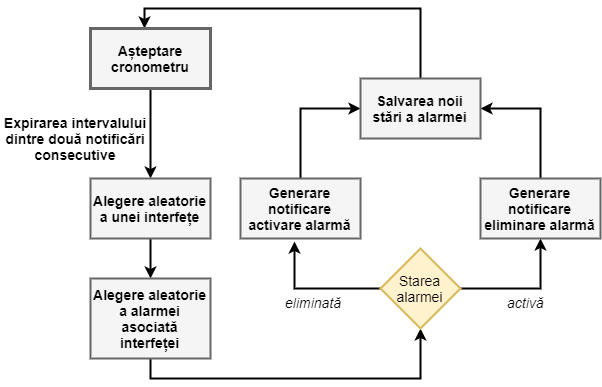
\includegraphics[width=1\textwidth]{wte_notif_generation}
	\caption{Organigrama mecanismului de generare a notificărilor NETCONF fictive al WTE.}
	\label{fig:wte_notif_generation}
\end{figure}

Până acum, generarea acestora se baza pe intervalul dintre două notificări consecutive definit în fişierul de configurare al \gls{dvm} și pe detaliile notificării ce se preluau din același loc. Acum, abordarea este diferită. În cazul notificărilor de tip \textit{valoarea atributului s-a schimbat - attributeValueChanged}, am modificat unealta care generează automat scheletul de cod C asociat serverului \gls{netconf}, astfel încât fiecare funcție cu apel invers asociată unui atribut configurabil va invoca funcţia ce trimite această notificare, conţinând valorile reale de care este nevoie: obiectul căruia i s-a schimbat valoare și noua valoare a acestuia. În acest mod, notificările de schimbare a valorii unui atribut nu mai sunt fictive, ci vor fi recepţionate de clienţii \gls{netconf} care s-au abonat la primirea acestora, chiar în momentul în care valoarea se schimbă. În cazul notificărilor de tip \textit{problemă - problemNotification}, sau alarmele pe care le generează dispozitivele de rețea, a fost păstrat principiul declanşării acestora în mod fictiv. Prin natura modelului informațional pentru microunde, fiecare interfață are asociată o listă de probleme pe care le poate avea și este definit și un număr minim de elemente pe care această listă să le aibă. \gls{wte} profită de acest aspect, implementând următorul mecanism de generare a alarmelor fictive: pentru fiecare problemă se retine starea acesteia: \textit{activă} sau \textit{eliminată}. Când intervalul dintre două notificări fictive consecutive s-a scurs, simulatorul se va pregăti să trimită o nouă notificare, astfel: se va alege în mod aleator o interfață a dispozitivului, iar din lista de probleme asociată interfeţei se va alege, din nou în mod aleator, o alarmă. În cazul în care starea acesteia este \textit{activă}, se trimite o notificare care conţine eliminarea acestei alarme și se schimbă starea asociată acestei probleme în \textit{eliminată}. Dacă starea acesteia era \textit{eliminată}, se va trimite o notificare care conţine activarea acestei probleme și starea ei va fi schimbată în \textit{activă}. Acest mecanism oferă dezvoltatorilor de aplicații \gls{sdn} un oarecare realism al simulatorului, alarmele fiind generate aleatoriu și, în cazul în care o alarmă era deja prezentă în echipamentul de control, există și posibilitatea ca această problemă să fie eliminată acum.

\subsection{Nucleul simulatorului WTE}

Nucleul simulatorului \gls{wte} reprezintă codul de bază ce oferă infrastructura care, împreună cu celelalte unelte software, furnizează funcţionalitatea propusă: emularea unei rețele de transport de date fără fir, în același timp expunând modelele informaționale dezvoltate de \gls{onf}, TR-532 și TR-512. Este implementat în limbajul Python, folosind o metodă orientată pe obiecte, fiind astfel flexibil și modular, oferind posibilitatea unei extinderi facile. Această abordare este similară cu cea folosită în cadrul celui mai important simulator pentru rețele definite prin software, \textit{mininet}. Asemănările, dar și motivele pentru care \gls{wte} nu a fost dezvoltat pe infrastructura oferită de \textit{mininet} vor fi detaliate în capitolul următor. Diagrama de clase a nucleului \gls{wte} este prezentată în Figura~\ref{fig:wte_class_diagram}.

\begin{figure}[h]
	\centering
	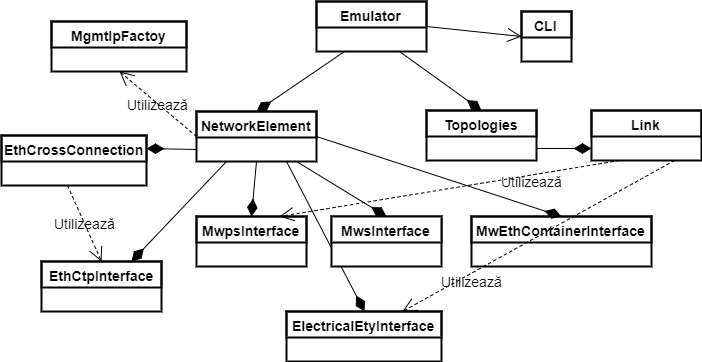
\includegraphics[width=1\textwidth]{wte_class_diagram}
	\caption{Diagrama de clase a nucleului WTE.}
	\label{fig:wte_class_diagram}
\end{figure}

Clasele proiectate pentru \gls{wte} sunt folosite în scopul reprezentării obiectelor care au o anumită semnificaţie în interiorul simulatorului. Astfel, clasa \textit{Emulator} este cea mai importantă, asigurând mediul în care toate celelalte instanţe ale obiectelor \gls{wte} vor fi create. Respectă modelul de programare obiect orientată \textit{Singleton}, însemnând că un singur obiect de acest tip va exista în momentul execuţiei programului. Este responsabilă de încărcarea și analizarea fişierelor \gls{json} de configurare a simulatorului. Parametrii din fişierul \textit{config.json} vor fi salvaţi ca variabile de execuţie, pentru a putea fi folosiţi ulterior. În cazul fişierului \textit{topology.json}, clasa \textit{Emulator} este responsabilă de analiza acestuia și de crearea obiectelor reprezentând elementele de rețea, respectiv legăturile de date dintre interfeţele acestora. Această clasă oferă și metode pentru executarea unor comenzi în maşina Linux sub care rulează \gls{wte}.

Clasa \textit{NetworkElement} este folosită pentru reprezentarea unui dispozitiv de rețea. În funcție de fişierul care descrie topologia, vor fi create mai multe instanţe ale acestei clase de către obiectul \textit{Emulator}. Atributele clasei sunt reprezentate, printre altele, de numele elementului de rețea, tipul acestuia (acest tip se referă de fapt la soluţia aleasă pentru implementarea serverului \gls{netconf} asociat, care poate fi \gls{dvm} sau altă variantă ce poate fi dezvoltată de către utilizator), lista conexiunilor Ethernet interne (reprezentând practic obiectele \gls{fc} din modelul informațional de bază), scheletul fişierului \gls{xml} care conţine atributele \gls{yang} configurabile, necesar pentru iniţializarea serverului \gls{netconf} și scheletul fişierului \gls{xml} care conţine atributele de stare, din care \gls{dvm} va returna valorile asociate acestora. Clasa \textit{NetworkElement} este responsabilă și pentru menținerea listei de obiecte reprezentând interfeţele pe care acel dispozitiv le prezintă. Oferă metode pentru crearea acestora, dar și pentru alterarea fişierelor \gls{xml} astfel încât să reflecte configurația definită de către utilizator în topologie. Celelalte metode importante pe care această clasă le oferă sunt în legătură cu lucrul cu containerul \textit{docker} asociat elementului de rețea: executarea de comenzi în interiorul containerul, iniţializarea containerului, copierea fişierelor \gls{xml} asociate \gls{dvm} în interiorul containerului \textit{docker}, etc.

Există mai multe clase care definesc obiecte de tip interfață a unui echipament de rețea, în funcție de tipul acestora. Tipul lor este dat de nivelul de transport specificat în modelul informațional de bază. Astfel, clasele asociate interfețelor de rețea sunt:
\begin{itemize}
	\item \textit{MwpsInterface} - asociată obiectelor \gls{ltp} de pe nivelul de transport \gls{mwps};
	\item \textit{MwsInterface} - asociată obiectelor \gls{ltp} de pe nivelul de transport \gls{mws};
	\item \textit{MwEthInterface} - asociată obiectelor \gls{ltp} de pe nivelul de transport \gls{etc};
	\item \textit{ElectricalEtyInterface} - asociată obiectelor \gls{ltp} de pe nivelul de transport \gls{ety};
	\item \textit{EthCtpInterface} - asociată obiectelor \gls{ltp} de pe nivelul de transport \gls{eth}.
\end{itemize}

Toate aceste clase oferă funcţionalitatea asociată unei interfețe, cu elementele specifice date de nivelul de transport la care operează (de exemplu relaţia client-server dintre obiectele \gls{ltp}, metode pentru alterarea fişierelor \gls{xml} asociate \gls{dvm} cu informații despre interfaţa respectivă, etc.).

Clasa \textit{Topology} reprezintă topologiile care se definesc în fişierul de configurare. Acestea pot fi prezente la două niveluri, \gls{mwps} și \gls{ety}. Aceste obiecte conţin de fapt obiectele de tip legătură, ce definesc topologia de rețea.

Clasa \textit{Link} reprezintă o legătură dintre două interfețe de rețea. Este responsabilă de stocarea celor două capete ce formează această legătură, dar și să valideze faptul că aceste capete sunt valide (există obiecte de tip interfață create anterior, între care se va putea face legătura efectivă). O metodă importantă pe care această clasă o oferă este cea responsabilă de crearea efectivă a legăturii (prin \gls{ovs} sau prin perechi Ethernet virtuale, așa cum va fi descris ulterior) dintre interfeţele de rețea Linux prezente în containerul \textit{docker}.

Figura~\ref{fig:wte_seq_diagram} prezintă o diagramă de secvenţă simplificată ce arată iniţializarea \gls{wte}.

\begin{figure}[h]
	\centering
	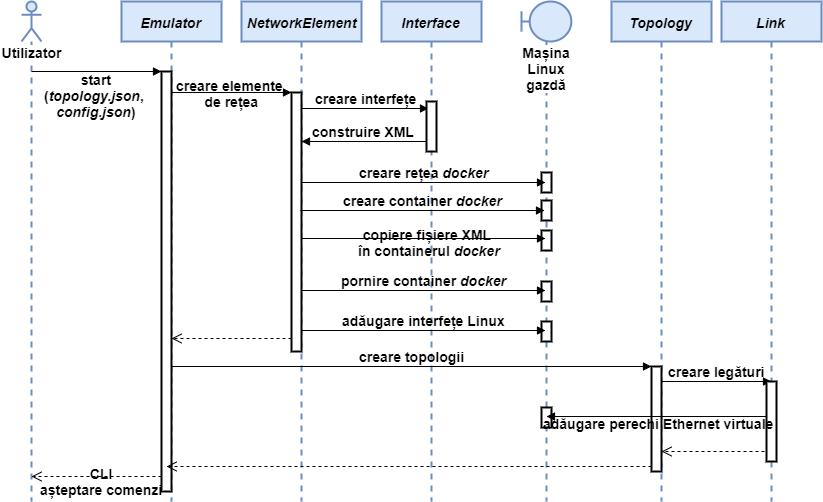
\includegraphics[width=1\textwidth]{wte_seq_diagram}
	\caption{Diagrama de secvenţă simplificată a inițializării WTE.}
	\label{fig:wte_seq_diagram}
\end{figure}

Construirea fişierelor \gls{xml} folosite de către \gls{dvm} este responsabilitatea fiecărui obiect dispozitiv de rețea, împreună cu interfeţele sale asociate. Fiecare obiect va altera modelul informațional adăugând informaţiile care îl reprezintă, astfel încât serverul \gls{netconf} să le pună la dispoziţie aplicațiilor \gls{sdn}. Apoi, aceste fişiere vor fi copiate în interiorul containerului \textit{docker} asociat și vor fi folosite de către \gls{dvm} pentru iniţializarea serverului \gls{netconf} și citirea valorilor atributelor de stare.

\subsection{Reprezentarea interfeţelor unui dispozitiv de rețea}

Fiecare interfață de rețea a echipamentelor, cu alte cuvinte fiecare obiect \gls{ltp} din modelul informațional de bază, indiferent de nivelul de transport pe care se află (\gls{mwps}, \gls{mws}, \gls{etc}, \gls{ety}, \gls{eth}), va fi reprezentată ca o interfață Linux, în interiorul containerului \textit{docker} asociat fiecărui dispozitiv de rețea. Legăturile interne din acest container, între interfeţele de rețea, vor fi descrise în paragrafele următoare. Pentru o mai bună înţelegere, acestea sunt prezentate în Figurile \ref{fig:wte_ltp_relationship} și \ref{fig:wte_ltp_ne_internal}.

\begin{figure}[h]
	\centering
	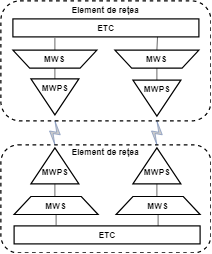
\includegraphics{wte_ltp_relationship}
	\caption{Obiectele LTP în contextul legăturii dintre două dispozitive de transport de date fără fir.}
	\label{fig:wte_ltp_relationship}
\end{figure}

\begin{figure}[h]
	\centering
	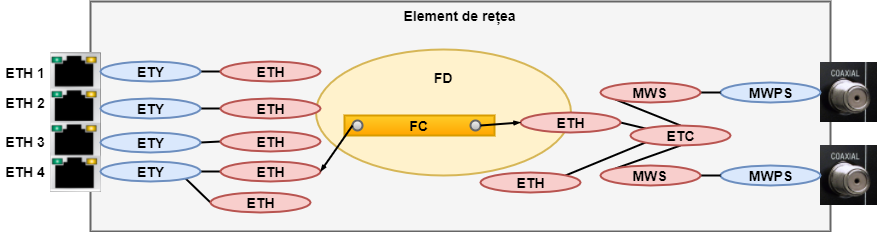
\includegraphics[width=1\textwidth]{wte_ltp_ne_internal}
	\caption{Obiectele LTP în interiorul unui dispozitiv de transport de date fără fir.}
	\label{fig:wte_ltp_ne_internal}
\end{figure}

Toate obiectele \gls{ltp} vor fi adăugate ca interfețe Linux având drept nume identificatorul unic universal asociat acestuia, așa cum este definit de către utilizator în fişierul de topologie al simulatorului. Adăugarea se va face cu ajutorul utilitarului \textit{\textbf{ip}}, oferit de Linux. Obiectele \gls{ltp} care se află la nivelurile \gls{mwps} sau \gls{ety} reprezintă interfețe ale dispozitivului de rețea cu exteriorul (radio, respectiv Ethernet). Astfel, dacă nu sunt definite legături în topologie care să utilizeze obiectul respectiv, acesta va fi reprezentat în containerul \textit{docker} drept o \textit{interfață fictivă de rețea (dummy interface)}. Adăugarea obiectului în Linux, în cazul în care acesta face parte dintr-o legătură va fi descrisă în sub-secţiunea următoare.

Obiectele \gls{ltp} de pe celelalte niveluri de transport vor avea, obligatoriu, o relaţie de tip client-server. Relaţiile, așa cum sunt definite în modelul informațional pentru microunde, sunt următoarele: obiectele de pe nivelurile \gls{mwps} și \gls{ety} nu își pot asuma rolul de client. Un obiect \gls{ltp} de pe nivelul \gls{mws} va avea drept server un obiect \gls{ltp} de pe nivelul \gls{mwps}, în timp ce un obiect \gls{ltp} de pe nivelul \gls{etc} va avea drept server un obiect \gls{ltp} de pe nivelul \gls{etc}. Obiectele \gls{ltp} de pe nivelul \gls{eth} pot avea ca server obiecte \gls{ltp} de pe nivelurile \gls{etc} sau \gls{ety}. Figura \ref{fig:wte_ltp_ne_internal} prezintă aceste legături. Soluția pentru reprezentarea acestor relaţii de tip client-server în Linux este folosirea interfeţelor de tip \textit{legătură (bond)}. O interfață de tip \textit{legătură} este o conexiune logică ce poate agrega mai multe interfețe. În acest mod, putem privi conexiunea logică, sau agregatorul, ca fiind clientul, iar interfeţele care sunt agregate ca fiind serverul. Considerând exemplul din Figura \ref{fig:wte_ltp_relationship}, pentru un element de rețea, obiectele \gls{ltp} de pe nivelul \gls{mws} vor fi reprezentate ca interfețe de tip \textit{legătură}, care agregă o singura interfață fiecare, dintre cele asociate obiectelor \gls{ltp} de pe nivelul \gls{mwps}, în timp ce obiectul \gls{ltp} de pe nivelul \gls{etc} va fi reprezentat printr-o interfață de tip \textit{legătură} ce va agrega cele două interfețe logice create pentru obiectele \gls{ltp} de pe nivelul \gls{mws}. Există mai multe moduri de funcţionare pentru interfeţele de tip \textit{legătură}, dar cel ales pentru \gls{wte} este acela în care distribuţia traficului pe conexiunile ce fac parte din acestă interfață logică este una simplă: conexiunile agregate sunt iterate și li se transmite câte un pachet de date, pe rând (\textit{round-robin}).

Obiectele \gls{ltp} de pe nivelul \gls{eth} sunt reprezentate ca interfețe virtuale de tip \textit{vlan}. Deoarece acestea au obligatoriu un identificator \gls{vlan} asociat, unei interfețe care reprezintă obiecte \gls{ltp} de pe nivelurile \gls{ety} sau \gls{etc} i se va putea asocia o interfață virtuală ce va semnifica obiectul \gls{ltp} de pe nivelul \gls{eth}.

Reprezentarea obiectelor de tip conexiuni Ethernet (\gls{fc}) este diferită față de celelalte. În acest caz, legătura dintre două obiecte de tip \gls{ltp} de pe nivelul \gls{eth} se face printr-o interfață logică de tip \textit{bridge}. Acesteia i se adaugă cele două interfețe de tip \textit{vlan} ce reprezintă cele două capete ale conexiunii Ethernet, astfel traficul va fi dirijat, prin interfaţa de tip \textit{bridge}, între acestea.

\subsection{Legăturile dintre interfeţele elementelor de rețea}

Au existat două abordări pentru reprezentarea legăturilor dintre elementele de rețea: prima metodă consta în realizarea unor conexiuni între două interfețe printr-un comutator software \gls{ovs}, iar cea de-a doua în crearea unei legături logice între două interfețe prin perechi Ethernet virtuale (\textit{veth pairs}). Cea din urmă a fost aleasă pentru implementare, însă vor fi prezentate ambele metode, pentru a înţelege de ce am făcut această alegere. Abordările considerate sunt ilustrate în Figura \ref{fig:wte_link_representation}.

\begin{figure}[h]
	\centering
	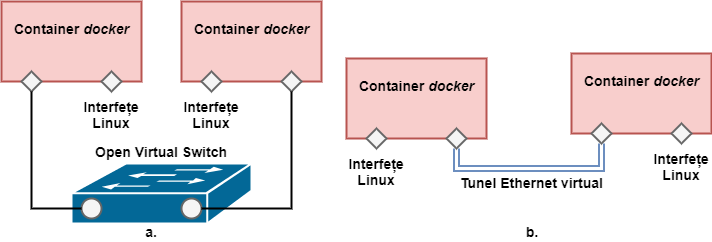
\includegraphics[width=1\textwidth]{wte_link_representation}
	\caption{Legăturile dintre interfeţele elementelor de rețea considerate pentru WTE: a) prin OVS; b) prin perechi Ethernet virtuale}
	\label{fig:wte_link_representation}
\end{figure}

Prima soluție considerată pentru reprezentarea legăturilor dintre interfeţele elementelor de rețea a fost prin intermediul unui comutator software \gls{ovs}. Astfel, pentru fiecare legătură trebuia creat un comutator \gls{ovs}, la care cele două capete ale legăturii (câte unul în fiecare container \textit{docker} asociat elementului de rețea) trebuiau legate. Ar fi fost posibilă și crearea unui singur comutator \gls{ovs} care să cuprindă toate legăturile din topologie, însă apoi trebuiau implementate restricţii la nivelul acestuia, pentru a nu exista legături nedorite (între alte interfețe decât cele specificate în fişierul de topologie). Modelarea legăturii fără fir era posibilă prin aplicarea unor restricţii de calitate de servicii - \gls{qos} asupra conexiunii respective, în interiorul comutatorului \gls{ovs} (de exemplu lărgimea de bandă să fie una specifică unei legături între echipamente de transport de date fără fir). Această abordare prezenta însă un dezavantaj major. Presupunând că o interfață Linux dintr-un container \textit{docker} ar fi fost dezactivată, era de așteptat ca acest lucru să fie vizibil și în celălalt capăt al legăturii și interfaţa îndepărtată să raporteze o stare operaţională \textit{închisă}. Deoarece legătura era făcută prin comutatorul software \gls{ovs}, acest lucru nu s-ar fi întâmplat, pentru că stările porturilor din comutator sunt independente și nu s-ar fi propagat între porturile prin care se face conexiunea. Acest dezavantaj major a condus la căutarea unei alte soluții pentru reprezentarea acestor legături. O altă problemă pe care această abordare o ridică este consumul de resurse. Fiecare legătură va avea propriul comutator \gls{ovs} asociat, astfel că pentru o topologie de rețea cu multe conexiuni, va exista un consum de resurse nejustificat de mare. De asemenea, instalarea \gls{wte} pe maşina Linux gazdă va fi mai greoaie, deoarece ar implica și instalarea prealabilă a \gls{ovs}.

Răspunsul la provocările menţionate anterior constă în următorul concept pus la dispoziţie de Linux: perechi Ethernet virtuale. Acestea reprezintă perechi de interfețe virtuale Linux de rețea care sunt conectate printr-un \textit{tunel}. Tot traficul care va intra într-o interfață va fi dirijat către interfaţa pereche, ca și când acestea ar fi conectate printr-un cablu Ethernet virtual. În cazul \gls{wte}, în momentul în care se încearcă reprezentarea unei legături din fişierul de topologie, o astfel de pereche este creată. Apoi, un capăt al conexiunii va fi asociat containerului \textit{docker} asociat primului dispozitiv de rețea al legăturii, iar celălalt capăt celui de-al doilea container \textit{docker}. În acest mod, în momentul în care una dintre interfețe este dezactivată, acest lucru se va propaga imediat la interfaţa îndepărtată, care va raporta o stare operaţională \textit{închisă}. Modelarea unei legături fără fir se poate face în mod facil folosind această abordare. Linux oferă utilitarul \textit{\textbf{tc}} - Traffic Control. Acesta poate instrui nucleul sistemului de operare să altereze caracteristicile unei interfețe virtuale, precum: debitul interfeţei, latenţa pe care interfaţa o introduce în traficul pe care îl transportă, procentul de pachete pe care interfaţa de poate pierde, etc.

Pe baza considerentelor expuse anterior, a fost implementată ce-a de-a doua soluție pentru reprezentarea legăturilor dintre interfeţele echipamentelor de rețea: folosirea perechilor Ethernet virtuale.

\subsection{Modelarea conexiunilor dintre dispozitivele simulate ca legături fără fir}

O parte importantă a \gls{wte}, care este reprezentativă pentru considerarea acestuia ca fiind un simulator de rețele de transport de date fără fir, nu doar o unealtă care expune modelele informaționale dezvoltate de \gls{onf} conform cu fişierul în care este definită topologia, este dată de modelarea conexiunilor dintre dispozitivele de rețea simulate având caracteristicile unei legături fără fir.

Caracteristicile ce pot fi alterate prin unealta \textit{\textbf{tc}} oferită de Linux, care sunt relevante pentru simularea unei legături fără fir, sunt reprezentate de debitul interfeţei, întârzierea pachetelor ce tranzitează această conexiune și procentul de pachete pierdute.

Debitul unei interfețe este influenţat de mai mulți parametri, dintre care unii sunt configurabili. TR-532 oferă și o formulă de calcul pentru acest debit, tocmai pentru ca aplicațiile \gls{sdn} ce se folosesc de acest model să fie aliniate asupra acestei metode. Ecuația \ref{eq:txCapacityFormula} descrie această metodă de calcul.

\begin{equation}\label{eq:txCapacityFormula}
\begin{split}
txCapacity& =AirInterface::AirInterfaceConfiguration::\textbf{\textit{txChannelBandwidth}}\\
& \quad * \log_{2}(AirInterface::AirInterfaceStatus::\textbf{\textit{modulationCur}})\\
& \quad * AirInterface::AirInterfaceStatus::\textbf{\textit{codeRateCur}} * 0,85
\end{split}
\end{equation}
unde:

$txCapacity$ = debitul interfeţei de rețea, în kbps

$txChannelBandwidth$ = lărgimea de bandă a emiţătorului, în kHz

$modulationCur$ = schema de modulaţie folosită, în număr de simboluri

$codeRateCur$ = procentul informaţiei utile din informaţia transmisă\\

Rata de transmisie a încărcăturii utile, reprezintă produsul dintre rata de transmisie brută și procentul informaţiei utile din informaţia transmisă ($codeRateCur$), unde acesta reprezintă numărul de biţi ai încărcăturii utile, raportat la numărul total de biţi transmişi. Acest procent apare din cauza redundanţei introduse pentru corectarea de erori și alte informații care nu fac parte din încărcătura utilă și are o valoare tipică între 0,85 și 0,95~\cite{kizer2013digital}. În cazul \gls{wte}, am considerat valoarea acestei rate curente a codului ca fiind 0,9.

Rata de transmisie brută este definită ca produsul dintre rata simbolurilor și numărul de biţi per simbol. Valoarea acestuia din urmă este dată de modulaţia folosită la transmisie. Modulaţia tipică folosită în echipamentele de transport de date fără fir este Modulaţia de Amplitudine în Cuadratură - \gls{qam}. În acest caz, numărul de biţi per simbol este definit ca $\log_{2}$ din numărul de constelaţii (reprezentat în modelul informațional prin $modulationCur$). Rata simbolurilor tipică pentru acest tip de echipamente este de aproximativ 85\% din lărgimea de bandă ($txChannelBandwidth$) a canalului de transmisie~\cite{kizer2013digital}.

Această formulă este implementată în cadrul \gls{wte}. În momentul în care unul dintre atributele unei interfețe pe baza cărora se face calculul se schimbă (de exemplu o aplicație \gls{sdn} modifică lărgimea de bandă folosită de o interfață a unui echipament, sau modulaţia care se folosește pentru transmisie), instanţa \gls{dvm} asociată dispozitivului de rețea va calcula debitul interfeţei respective și apoi va folosi utilitarul Linux \textit{\textbf{tc}} pentru a modifica această caracteristică a interfeţei. În acest mod, legăturile fără fir vor fi modelate în simulator astfel încât să semene cu cele din rețelele reale, din punctul de vedere al ratei de transmisie.

În legătură cu latenţa pe care o introduc echipamentele de transport de date fără fir, tipic aceasta este de ordinul zecilor sau sutelor de microsecunde~\cite{kizer2013digital}. Această plajă de întârzieri nu pot fi simulate în cadrul \gls{wte}, deoarece utilitarul \textit{\textbf{tc}} oferă modificarea latenţei unei interfețe de rețea doar cu o rezoluţie de o milisecundă. Pentru a putea beneficia de rezoluţii mai mici, de ordinul microsecundelor, imaginea sistemului de operare Linux din containerul \textit{docker} ar trebui modificată și nucleul sistemului de operare recompilat, astfel încât să permită utilizarea unor cronometre de sistem de timp real. Versiunea curentă a \gls{wte} nu implementează acest comportament, dar acesta poate constitui subiectul unei alte cercetări, pentru a modela legăturile dintre interfeţele dispozitivelor de rețea simulate cât mai aproape de realitate.

Alterarea procentului de pachete pierdute de o interfață de rețea nu este încă folosit în \gls{wte}, deoarece presupunem că legătura fără fir este realizată în condiţii atmosferice optime, astfel încât să nu se piardă pachete. Ar putea fi totuşi utilizat, spre exemplu prin expunerea unei comenzi în linia de comandă a simulatorului, care să crească sau să scadă acest procent pentru o conexiune. Astfel, s-ar putea simula condiţii atmosferice potrivnice în anumite părţi ale topologiei de rețea. În acest mod ar putea fi testată, de exemplu, o aplicație \gls{sdn} care să detecteze faptul că există probleme în rețea (din cauza unei furtuni se pierd pachete, sau scade modulaţia folosită la emisie) și să dirijeze traficul prin altă parte a topologiei.

\subsection{Linia de comandă}

\gls{wte} dispune de un modul care oferă o interfață prin linie de comandă utilizatorului. După ce acesta porneşte simulatorul, la sfârşitul inițializării (adică după ce au fost create toate obiectele asociate cu topologia de rețea specificată în fişierul de configurare) se lansează modulul care implementează interfaţa prin linie de comandă - \gls{cli}. Acesta oferă utilizatorului posibilitatea unei interacţiuni simple cu simulatorul, prin furnizarea unor comenzi clare, simplu de folosit. O captură de ecran a acestei interfețe este prezentată în Figura \ref{fig:wte_cli_screenshot}.

\begin{figure}[h]
	\centering
	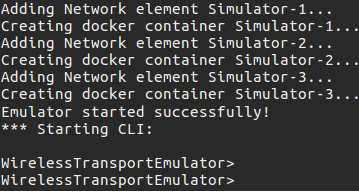
\includegraphics{wte_cli_screenshot}
	\caption{Captură de ecran a interfeţei prin linie de comandă a WTE.}
	\label{fig:wte_cli_screenshot}
\end{figure}

Comenzile implementate sunt următoarele:
\begin{itemize}
	\item \textit{afişare noduri} - afişează pe ecran numele tuturor dispozitivelor de rețea simulate;
	\item \textit{afişare informații nod} - afişează pe ecran toate informaţiile disponibile despre un anumit echipament de rețea simulat: nume, adresa \gls{ip} a interfeţei de administrare, portul folosit de serverul \gls{netconf}, lista interfeţelor nodului respectiv împreună cu nivelul de transport pe care acesta se află;
	\item \textit{afişare legături} - afişează pe ecran toate legăturile dintre interfețe prezente în topologia simulată, inclusiv nivelul de transport la care este realizată aceasta (\gls{mwps} sau \gls{ety});
	\item \textit{pornire terminal} - porneşte un terminal care se leagă la containerul \textit{docker} asociat unui element de rețea, oferind acces la mediul Linux din interiorul imaginii. Acesta poate fi folosit de utilizator pentru a interacţiona într-un mod facil și direct cu elementul de rețea respectiv.
	\item \textit{înregistrare / anularea înregistrării \gls{odl}} - această comandă oferă posibilitatea de a înregistra / anula înregistrarea în mod automat pentru elementele de rețea la / de la echipamentul de control \gls{sdn} (în particular \gls{odl}). Detaliile de conectare la echipamentul de control \gls{sdn} sunt cele specificate în fişierul de configurare al \gls{wte};
	\item \textit{închidere} - această comandă poate fi folosită de către utilizator pentru închiderea simulatorului (împreună cu toate obiectele pe care acesta le-a creat în interiorul maşinii Linux gazdă).
\end{itemize}

\subsection{Generarea traficului de date}

Pentru a oferi o soluție completă de simulare, inclusiv validarea topologiei și a legăturilor create, \gls{wte} pune la dispoziţie utilizatorilor și posibilitatea de a genera trafic de date între anumite puncte ale rețelei. În acest scop este folosită unealta software \textit{iperf3} \cite{iperf32017, tirumala2005iperf}. Aceasta este instalată în sistemul de operare Linux din imaginea \textit{docker} folosită de fiecare dispozitiv de rețea simulat.

Toate conexiunile descrise până acum sunt făcute la nivelul 2 (legătură de date) din stiva \gls{osi}. Astfel, interfeţele Linux din containerul \textit{docker} nu folosesc adrese \gls{ip} (în afară de cea de administrare). Generarea de trafic se face între două interfețe, una jucând rolul de client, iar cealaltă de server. Pentru ca unealta \textit{iperf3} să poată funcţiona, este nevoie de adăugarea de adrese \gls{ip} celor două interfețe. \gls{wte} poate face acest lucru în mod automat, dacă în fişierul care descrie topologia, obiectului \textit{conexiune Ethernet} i se adaugă un atribut \textit{gazdă}. Astfel, acelui obiect i se asociază, la nivel teoretic, un port capabil să genereze sau să recepţioneze trafic. Practic, o adresă \gls{ip} este adăugată la interfaţa asociata acelui obiect. Apoi, utilizatorul va putea genera trafic între oricare două astfel de porturi. 

Unealta \textit{iperf3} permite generarea de trafic \gls{tcp} sau \gls{udp}, oferind în același timp posibilitatea de a măsura latenţa pachetelor, variaţia acestei latenţe (\textit{jitter}) sau lărgimea de bandă a canalului de comunicaţie folosit.

\subsection{Generarea adreselor IP de administrare și înregistrarea la controlerul ODL}

Pentru o simulare cât mai fidelă a rețelelor de transport de date fără fir, fiecare dispozitiv simulat va avea o interfață de administrare, prin care echipamentul de control \gls{sdn} (în particular \gls{odl}, care a fost folosit în demonstraţiile de concept \gls{onf}). Există două variante abordate în \gls{wte} pentru a identifica în mod unic o astfel de interfață și utilizatorul poate alege între acestea prin fişierul de configurare. În cazul în care atributul \textit{simulare bazată pe port} are valoare logică adevărată, interfeţelor de administrare ale elementelor simulate vor avea aceeaşi adresă \gls{ip}, dar vor fi diferenţiate prin port. Altfel, fiecare interfață va avea o adresă \gls{ip} diferită și același port. Alocarea acestor adrese \gls{ip} va fi descrisă în continuare.

Un exemplu de alocare a adreselor \gls{ip} de administrare este ilustrat în Figura \ref{fig:wte_management_ip}, pentru două dispozitive de rețea simulate.

\begin{figure}[h]
	\centering
	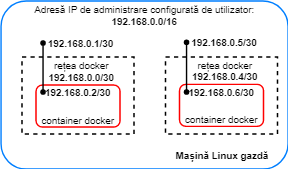
\includegraphics{wte_management_ip}
	\caption{Exemplu de alocare a adreselor IP de administrare pentru două elemente simulate.}
	\label{fig:wte_management_ip}
\end{figure}

Utilizatorul specifică, în fişierul de configurare al simulatorului, plaja de adrese destinată interfeţelor de administrare. Să presupunem că aceasta este \texttt{192.168.0.0/16}, conform figurii anterioare. Pentru ca echipamentul de control \gls{sdn} să poată accesa dispozitivele simulate, este necesar ca și adresa lui \gls{ip} să fie din același spațiu. Nucleul \gls{wte} va folosi această plajă de adrese pentru generarea de adrese \gls{ip} pentru interfeţele de administrare, prin obiectul \textit{MgmtIpFactory} (fabrică de adrese \gls{ip} de administrare). Acesta va împărţi spaţiul de adrese în sub-rețele având masca \texttt{/30}. Fiecărui element de rețea simulat i se va aloca o astfel de sub-rețea. În momentul creării rețelei \textit{docker} asociate echipamentului, aceasta va folosi adresa de rețea pusă la dispoziţie de fabrica de adrese \gls{ip} de administrare. A fost aleasă masca de rețea \texttt{/30}, deoarece aceasta pune la dispoziţie două adrese \gls{ip} pentru a putea fi folosite (celelalte două reprezintă adresa de rețea și adresa de difuzare generală - \textit{broadcast}). Aceste două adrese vor fi folosite de interfața de rețea din sistemul de operare Linux gazdă și respectiv interfața de rețea din interiorul containerului \textit{docker} asociat dispozitivului de rețea. Reluând exemplul anterior, dacă trebuie simulate două echipamente, rețelele \textit{docker} asociate vor fi: \texttt{192.168.0.0/30}, respectiv \texttt{192.168.0.4/30}, iar elementele simulate vor putea fi accesibile din exterior (echipamentul de control \gls{sdn}, de exemplu), prin adresele \gls{ip} \texttt{192.168.0.1}, respectiv \texttt{192.168.0.5}, însă nu va exista conectivitate între aceste interfețe, fiind în rețele diferite. Conectivitatea dintre echipamentele simulate va fi asigurată, în funcție de topologie, prin celelalte interfețe ce reprezintă porturi fără fir sau Ethernet.